\documentclass[a4paper,11pt]{article}

% Mise en page française
\usepackage[utf8]{inputenc}
\usepackage[french]{babel}
\usepackage{geometry}

% Import d'images, couleurs
\usepackage{graphicx,color}
\usepackage{multirow}


% Entêtes
\usepackage{fancyhdr}
\pagestyle{fancy}
\lhead{Cahier des charges}
\rhead{{RBLT-Corp}\\{Upside Down}}   

\usepackage{lipsum}

\newcommand{\hsp}{\hspace{20pt}}
\newcommand{\HRule}{\rule{\linewidth}{0.5mm}}





\begin{document}  


\begin{titlepage}
  \begin{sffamily}
  \begin{center}

  
    
\includegraphics[scale=0.3]{pictures/logo}~\\[1.5cm]

    \textsc{\LARGE EPITA Rennes}\\[0.5cm]

    % Titre
    \textsc{\Large Cahier des charges}\\[1.5cm]

    \HRule \\[0.4cm]
     { \huge \bfseries Upside Down \\[0.4cm] }

    \HRule \\[1.5cm]
    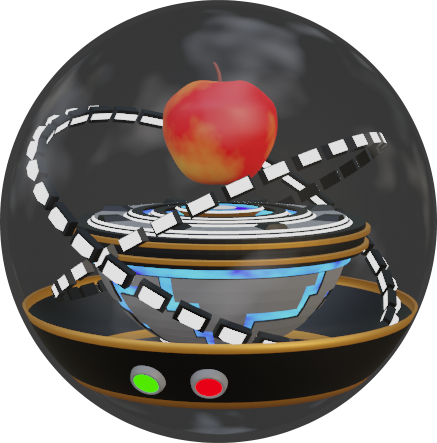
\includegraphics[scale=0.3]{pictures/Gravi.png}
     \\[0.5cm]
    \textsc{\Large RBLT-Corp}\\[1.5cm]

    % Membres
    \begin{minipage}{0.4\textwidth}
      \begin{flushleft} \large
        Ronan Leboucher\\
        Brian Perret\\
      \end{flushleft}
    \end{minipage}
    \begin{minipage}{0.4\textwidth}
      \begin{flushright} \large
        Lorenzo Lombardi\\
        Thomas Morin\\
      \end{flushright}
    \end{minipage}

    \vfill

    % Bottom of the page
    {\large 13 Janvier 2023}

  \end{center}
  \end{sffamily}
\end{titlepage}


\newpage

\tableofcontents

\newpage


\section{Introduction}

Le projet "Upside Down", un jeu vidéo qui sera développé par le groupe RBLT-Corp lors 
du second semestre à Epita.\newline

Le domaine du jeu vidéo est en constante évolution de par le développement des technologies
offrant des capacités et des rendu graphique à couper le souffle, mais aussi l'innovation des
mécaniques de jeu offrant aux joueurs de nouveaux défis.
Que ce soit tout seul, avec ses amis ou des parfait inconnues, cet essor permet ainsi d'avoir 
un vaste choix pouvant ravir tous les joueurs petits ou grands.\newline

Cependant en étant autant diversifié, cela créé de la concurrence entre les créateurs et il devient
donc difficile de se démarquer.
Avec cette idée en tête, notre groupe RBLT-Corp, composé de Ronan Leboucher, Lorenzo Lombardi, Brian Perret et Thomas Morin de R1, 
voulons proposer un jeu avec une mécanique de jeu innovante et très peu utilisé jusqu'ici. \newline

Deux joueurs devront coopérer pour résoudre une succession d'énigmes en manipulant le concept phare du jeu, la "gravité".
Ainsi les deux cerveaux devront travailler en tandem s'ils veulent passer à la salle suivante, car un joueur seul se retrouvera
dans l'incapacité de finir le jeu. Pour cela, ils auront à disposition un objet pouvant changer leur propre gravité et celle d'objets
spéciaux se trouvant dans les salles d'énigmes.




\section{Origine et nature du projet}

\subsection{Origine :}

	L’idée principale vient du souhait de pouvoir avoir un jeu agréable à manipuler 
    et à jouer avec un concept simple et très ouvert, permettant d’avoir rapidement le concept fonctionnel et ainsi de pouvoir le développer sur de nombreux points pour offrir une meilleure expérience de jeu. Après une mise en commun de nos idées, nous avons décidé de faire un jeu d’énigmes en s’appuyant sur le modèle du jeu Portal correspondant à nos critères.	

    \subsection{Nature :}
	Upside Down est un jeu de réflexion et d'action en duo.
Le jeu consiste en une succession de séries d'énigmes que les joueurs doivent 
résoudre en utilisant le principe de changement de gravité, soit sur lui-même ou bien sur les objets indépendamment contrôlables avec la “gravi-sphère”, l’outil principal du jeu. Les joueurs sont mis au défi par une intelligence artificielle et doivent résoudre chacune des énigmes en faisant preuve de réflexion et d'entraide s'ils veulent revoir la liberté.

\section{Objet de l’étude}

\subsection{Intérêt du projet}
Ce projet permet de nous apporter de nombreuses connaissances du point de vue management, 
travail en équipe, programmation et gestion du temps d’un projet de moyen terme, 
grâce à l’utilisation de méthodes très utilisées comme la méthode Agile et des logiciels pour l’appliquer : \newline

\begin{itemize}
    \item Jira pour la planification des sprints et de la gestion du temps
    \item Github pour le partage du code
    \item Discord pour l’échange\newline
\end{itemize}

Ces mêmes compétences qui nous seront nécessaires non seulement 
l’année prochaine, mais aussi durant notre vie aussi bien personnelle que professionnelle.

\subsection{But}

Notre but dans ce projet est de réussir à appliquer la méthode Agile, dans l’objectif 
de réaliser notre projet comme il a été prévu et dans les délais imposés.
Pour cela, nous allons découper notre projet en sous-projet (sprint).
Chaque sous-projet est constitué d’un ensemble de tâches attribuées à une ou plusieurs 
personnes qu’il faut réaliser. Une fois les tâches réalisées, notre projet sera au stade 
prévu par le sprint, nous pourrons donc passer au sprint suivant et ainsi de suite jusqu’à avoir le produit final.\newline

L'objectif d’établir un ensemble de sprints est que chacune des personnes du groupe sait 
où en est actuellement le projet et ce qu’il reste à faire sans être confronté à un océan de 
tâches à faire, mais seulement quelques tâches pour réaliser le sous-projet en cours.


\section{Etat de l’art}

\subsection{Modèle similaire}

Lors de la recherche du concept de base de notre jeu, nous avions pour modèle le très connu “Portal” 
qui a été extrêmement innovant pour un gameplay totalement inédit, ainsi que d’autre jeu du même type et 
de différentes époques comme “AntiChamber” (2013) ou encore “It takes two” (2021). 

\subsection{Fonctionnalité propre}

Nous avons donc tiré parti de ces jeux ce qui a fait leurs succès et leurs innovations appréciées des joueurs. C’est-à-dire, 
un concept basé sur un objet ou action offrant un gameplay original ( Générateur de portail, Géométrie non-euclidienne, … ) permettant de résoudre 
une suite d'énigmes totalement innovante grâce aux nouvelles mécaniques du concept de base, ainsi qu’une 
histoire associée permettant d’avoir une meilleure compréhension et immersion du jeu et de son intrigue.


\section{Gameplay}

\subsection{Descriptif d’une salle :} 

Deux joueurs se retrouvent dans une salle d'énigme, 
composée d’obstacles en tous genres ainsi que des éléments et actionneurs tels que des cubes 
à placer sur des plaques de pression pour actionner un mécanisme (porte, ascenseur, …) dans 
le but de rejoindre la fin du niveau. Pour arriver à leurs fins, les deux joueurs devront faire 
un certain nombre d’étapes en coopérant pour atteindre de nouvelles zones, plateformes.\newline

\subsection{Descriptif des joueurs :} 

Chacun des joueurs contrôle son propre avatar pouvant effectuer différentes actions : 
\newline

\begin{itemize}
    \item déplacement en 3 dimensions (sans double saut, ni dégât de chute)
    \item déplacer certains objets (cube, …)
    \item inversion de la gravité local du joueur et de l’item qu’il tient
    \item interaction avec les Personnage Non-Joueur pour connaître des indices \newline
\end{itemize}



Chaque joueur peut subir des dégâts et donc mourir uniquement via les différents pièges
 mis en place dans les salles d'énigmes.

Si un joueur vient à mourir, celui-ci réapparaît au début du niveau (au dernier point de sauvegarde) 

\section{L’intelligence artificielle}

\subsection{Présentation général :}

Une intelligence artificielle est mise en place sous la 
forme d’un Personnage-Non-Joueur nommé Monaco D. Whisky. 
Cette IA a pour rôle de donner des indices pour la prochaine salle d’énigme que les 
joueurs doivent réaliser à travers un certain nombre d’histoires concernant d’autres sujets de 
test qu’elle a pu rencontrer jusqu’alors.


\subsection{Spécifications de l’IA :}

L’IA se trouve dans la zone restreinte de son bar (qu’elle tient). Si le joueur cherche à 
interagir avec l’IA en se rapprochant de la zone, l’IA se rapprochera du comptoir où se trouve le joueur.\newline

Le joueur interagit avec l’IA sous forme de dialogue interactif (réponses multiples) 
en appuyant sur la touche associée et en étant au niveau du comptoir du bar.


\section{Répartition du travail}

\subsection{Répartition des rôles}

Nous avons répartit le travail en différent rôle en fonction des envies 
et des compétences de chacun :\newline

\begin{tabular}{ |p{3cm}|p{3cm}|p{3cm}|p{3cm}|  }
    \hline
    \multicolumn{4}{|c|}{Répartition des rôles} \\
    \hline
     Ronan & Brian & Lorenzo & Thomas\\
    \hline
     - Game Designer & - Chef de groupe & - Graphiste & - Game designer\\
     - Level designer & - Développeur & - Développeur & - Level designer\\
     - Scénariste & & & Scénariste\\
    \hline
\end{tabular}
\break
\newline

Ces choix ont été faits de telles sortes à ce que le projet est directement une bonne base, 
c’est-à-dire qu’il est préférable d’assigner le rôle à quelqu'un utilisant déjà le logiciel 
associé (exemple : Lorenzo créé de nombreux modèles 3D avec blender durant son temps libre ou encore
 Brian qui a déjà réalisé de multiples game jam avec Unity). Cela permet d'éviter de se retrouver à 
 apprendre un logiciel de zéro et 6 mois plus tard avec des bases de débutants qu’il faut entièrement refaire.
Et ainsi de permettre aux moins initiés de comprendre les bases et faire des applications avec 
moins de répercussions sur le projet en lui-même, tel que la création des salles et du scénario.

\subsection{Répartition des sprints}

Nous avons divisé notre projet en plusieurs sous-projet ou "sprint" selon le modèle Agile.
Chaque itération est constituéz d'un certain nombre de tâches à réaliser dans un temps que l'on fixe 
en fonction de leur complexité (Planning poker).\newline



\begin{tabular}{ |p{3cm}|p{3cm}|p{3cm}|p{3cm}|  }
 \hline
 \multicolumn{4}{|c|}{Liste des sprints jusqu'à mi-mai} \\
 \hline
 Objectif& Fonctionnalité de base  & Jeu fonctionnel & Histoire et Décoration\\
 \hline
 \hline
 Date fixée : & Mi-Février & Fin Mars & Mi-Mai\\
 \hline
 \multirow{3}{4em}{Fonctionnalité} & - Concept de base fonctionnel & - Toutes les salles sont fonctionnelles & - Dialogue\\ 
 & - Premières salles fonctionnelles & - Premières salles décorées & - Implémentation de l'IA\\ 
 & - Objets de base (cube, bouton, ...) & - Interface Utilisateur terminer & - Décoration des salles fini\\ 
 & & - Objets principaux fonctionnels & \\

 \hline
\end{tabular}


Le reste des sprints concernera principalement la recherche de bug et l'amélioration des 
fonctionnalités mineurs.



\section{Le réseau}

\subsection{Mode multijoueur :} 
	
Upside Down est fait pour être joué uniquement en duo. Unity offre plusieurs solutions très complètes, 
mais c’est “Mirror” qui a été choisi, principalement, car elle possède une très bonne documentation avec une 
grande communauté derrière tout en répondant aux contraintes de notre jeu, à savoir un besoin d’avoir une 
très faible latence entre les joueurs pour ne pas avoir de possibles décalages lors d’action rapide ainsi 
que de pouvoir lancer facilement des partie en local.


\subsection{Hébergement des services :}
	
L'hébergement des différents services (site web, multijoueur en ligne) se fera via le serveur 
que possède Brian permettant une plus grande flexibilité pour la maintenance des services.



\section{Coût opérationnel du projet}

Le coût du projet dépend de la charge sur les différents services.
Le service actuel est prévu pour encaisser une vingtaine de connexions simultanées.
En cas de plus forte demande, tous les services peuvent être installés chez un hébergeur tel que OVH. 
Ce coût de fonctionnement pouvant être amorti par la mise en place d’un prix d’achat par copie du jeu.


\section{Conclusion}

Nous sommes tous d'accord sur le sujet du jeu, et motivé pour le réaliser. Étant réalistes, nous espérons pouvoir le terminer
dans les délais prévus, mais avec l'utilisation de Jira, nous devrions n'avoir aucun problème à ce niveau-là.

Par ailleurs, le développement du jeu est déjà en cours où chacun travaille déjà sur son domaine attribué. Nous aspirons à surmonter les futures difficultés et de développer de nouvelles compétences et consolider celles déjà existante.
Enfin, nous désirons qu'aucun membre ne disparaisse durant ce semestre et qu'aucune tension ne vienne retarder l'avancement du projet.


\end{document}
